%% ======================================================================
%% 07_build.tex -- 6. Instrucciones de construccion
%% ======================================================================
\section{Instrucciones de construcción}
\label{sec:build}

\paragraph{Herramientas}
\begin{itemize}
  \item llaves hexagonales y llaves TETRIX;
  \item cautín, crimpadora para conectores XT60 y Dupont, multímetro y pinza amperimétrica de DC;
  \item impresora 3D FDM (PLA, capa de 0,2\,mm, 30\% de relleno para las torres y los mecanismos);
  \item una laptop con Arduino CLI (núcleo ESP32), PlatformIO y LabVIEW 2019 con el toolkit de myRIO.
\end{itemize}

\paragraph{Seguridad}
Ensamblar y grabar con las LiPo desconectadas y sin hélices. Comprobar el sentido de giro de cada motor sin hélices antes del primer vuelo.

\begin{figure}[!htbp]
  \centering
  \begin{subfigure}[b]{0.24\textwidth}\centering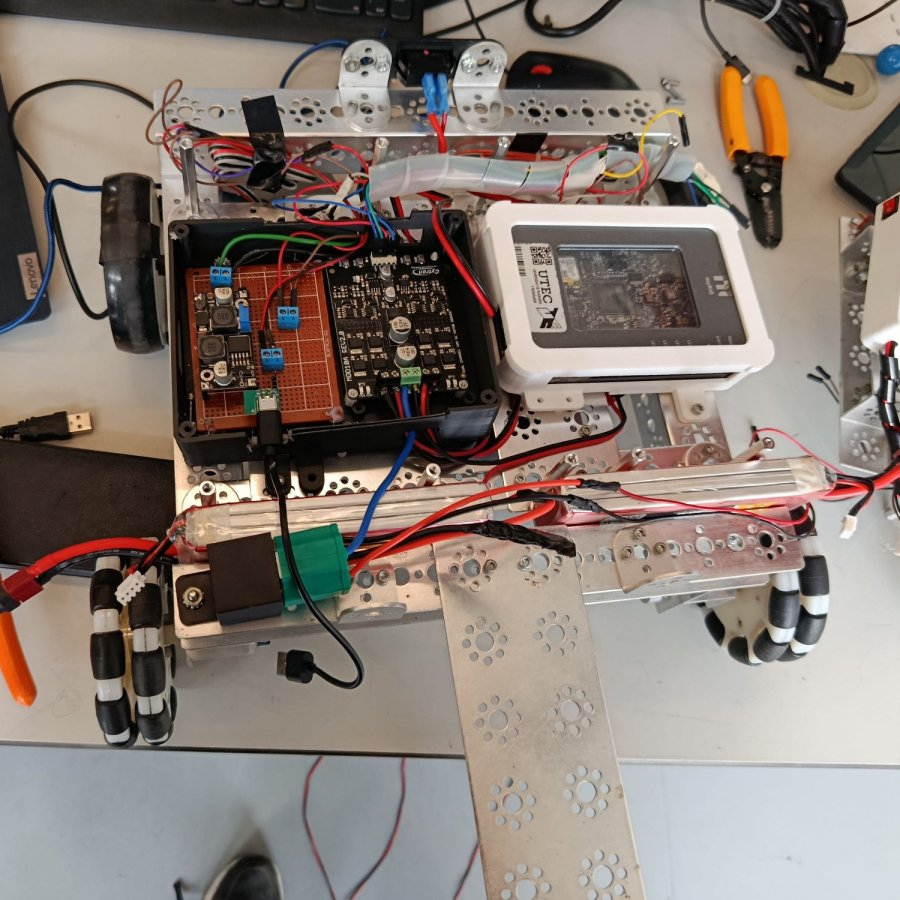
\includegraphics[width=\linewidth]{figures/paso1_base.jpg}\caption{Paso 1: base móvil (myRIO, MDD10A, LiPo).}\end{subfigure}\hfill
  \begin{subfigure}[b]{0.24\textwidth}\centering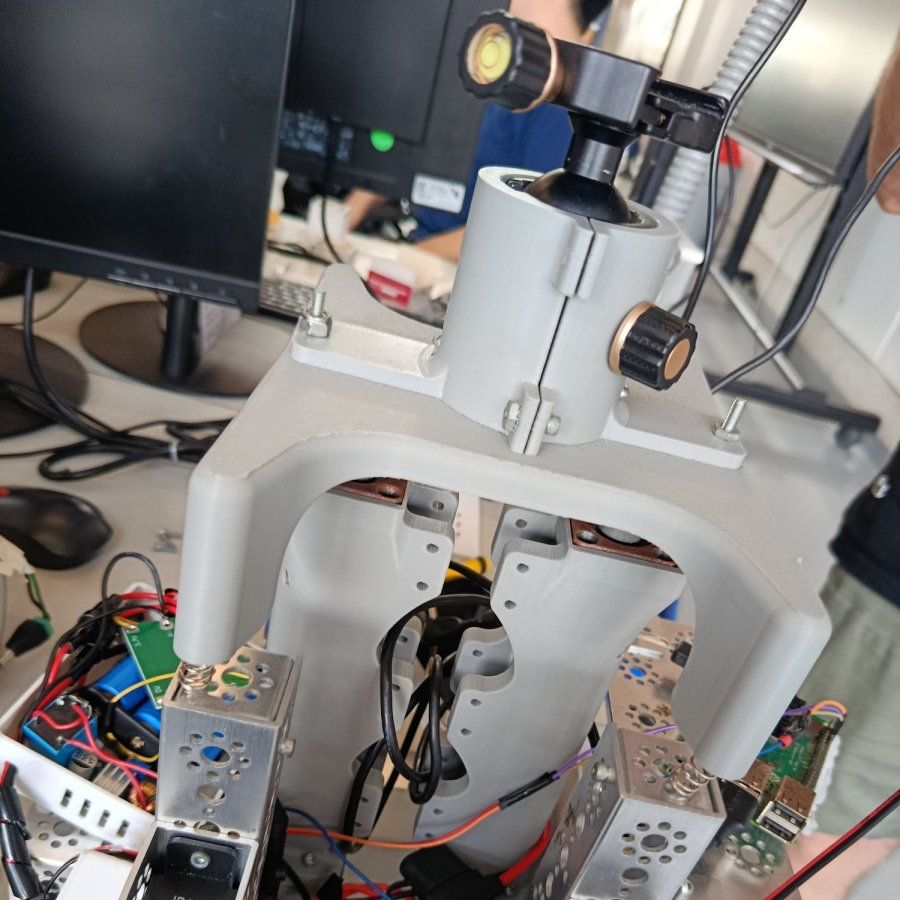
\includegraphics[width=\linewidth]{figures/paso2_mastil.jpg}\caption{Paso 2: mástil, guía y rótula.}\end{subfigure}\hfill
  \begin{subfigure}[b]{0.24\textwidth}\centering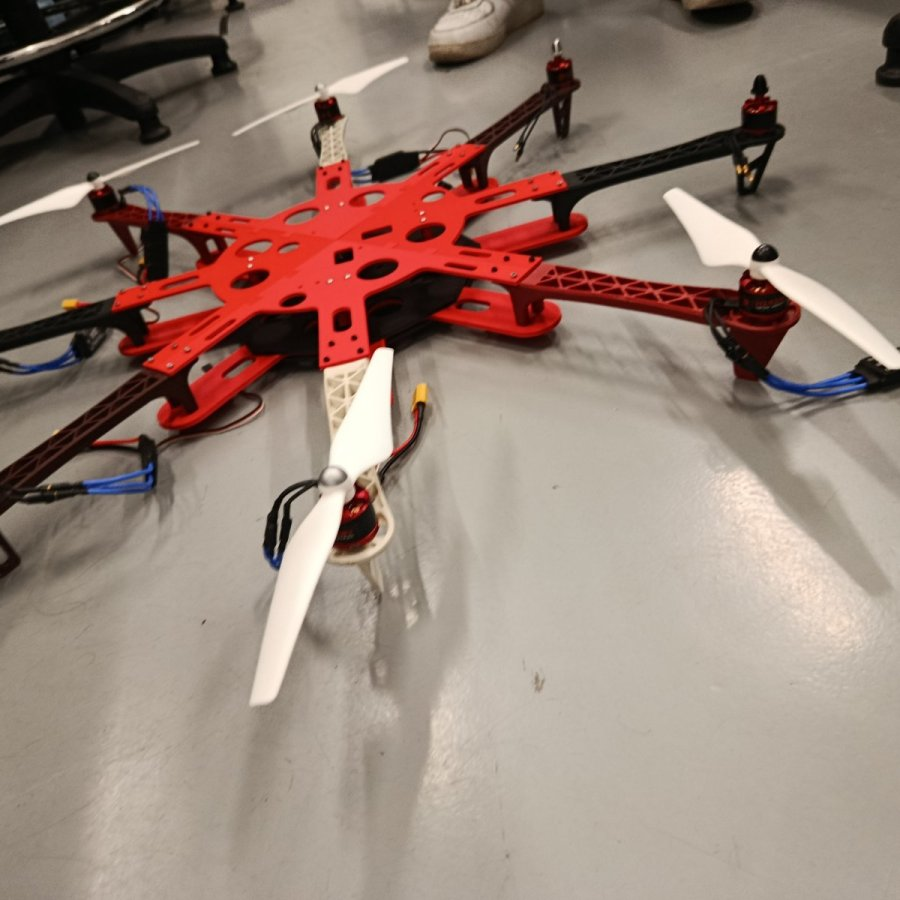
\includegraphics[width=\linewidth]{figures/paso3_marco.jpg}\caption{Paso 3: marco de ocho brazos.}\end{subfigure}\hfill
  \begin{subfigure}[b]{0.24\textwidth}\centering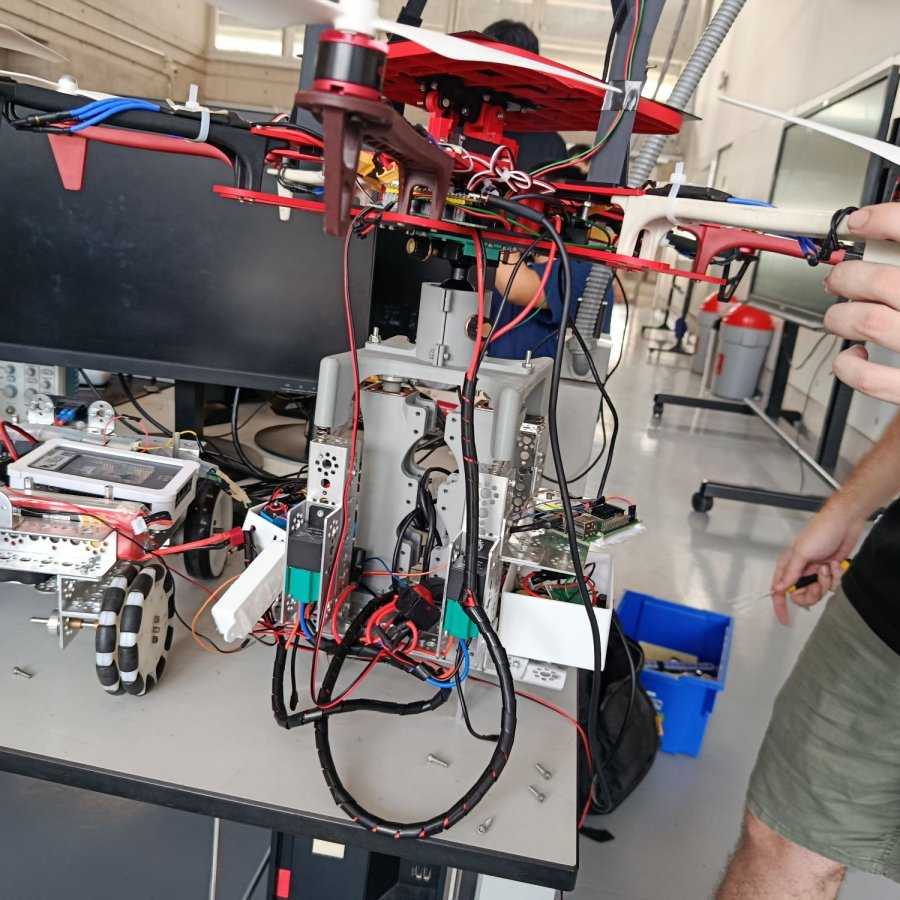
\includegraphics[width=\linewidth]{figures/paso4_dron_rotula.jpg}\caption{Paso 4: montaje del dron en la rótula.}\end{subfigure}\\[2mm]
  \begin{subfigure}[b]{0.24\textwidth}\centering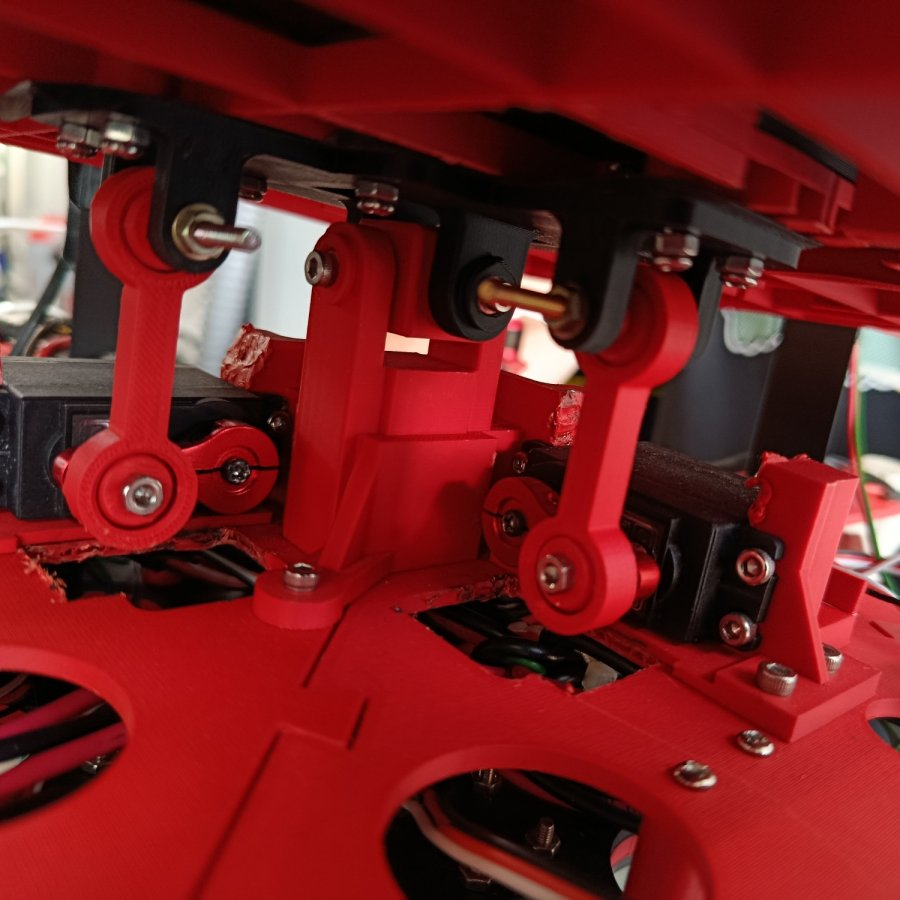
\includegraphics[width=\linewidth]{figures/paso5_mecanismo.jpg}\caption{Paso 5: servos y bielas de la bandeja.}\end{subfigure}\hfill
  \begin{subfigure}[b]{0.24\textwidth}\centering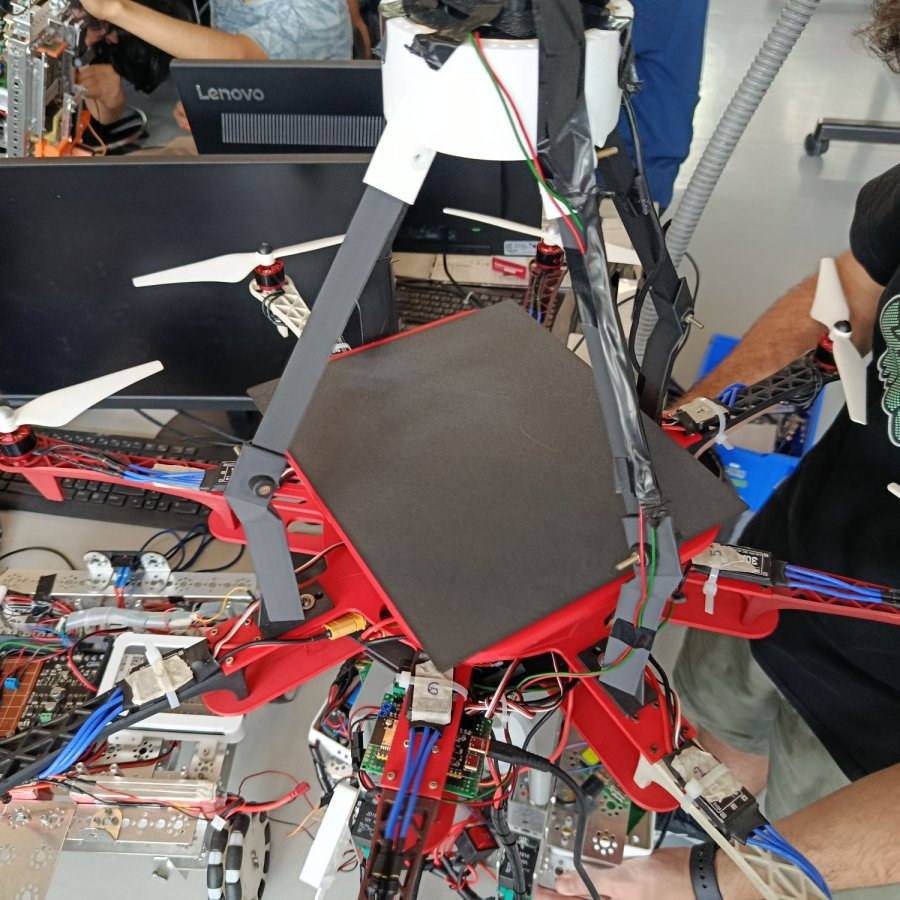
\includegraphics[width=\linewidth]{figures/paso5_bandeja_camara.jpg}\caption{Paso 5: plato y torres de la cámara.}\end{subfigure}\hfill
  \begin{subfigure}[b]{0.24\textwidth}\centering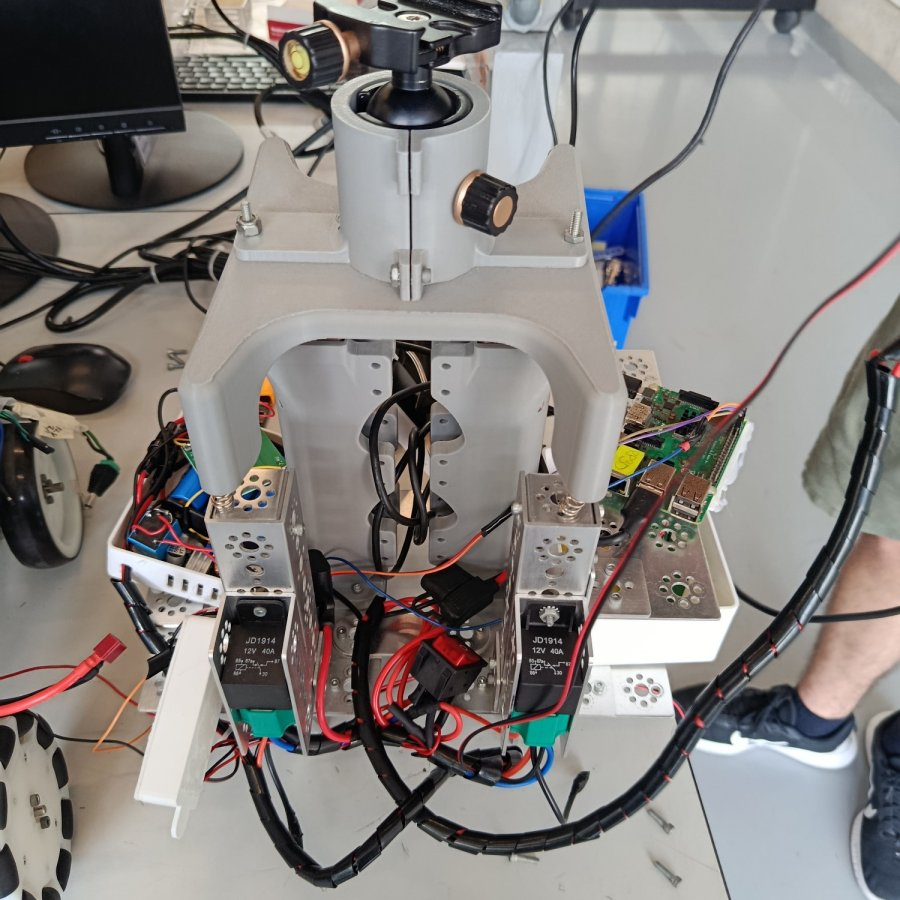
\includegraphics[width=\linewidth]{figures/paso6_supervisor.jpg}\caption{Paso 6: relés de paro y Raspberry Pi.}\end{subfigure}\hfill
  \begin{subfigure}[b]{0.24\textwidth}\centering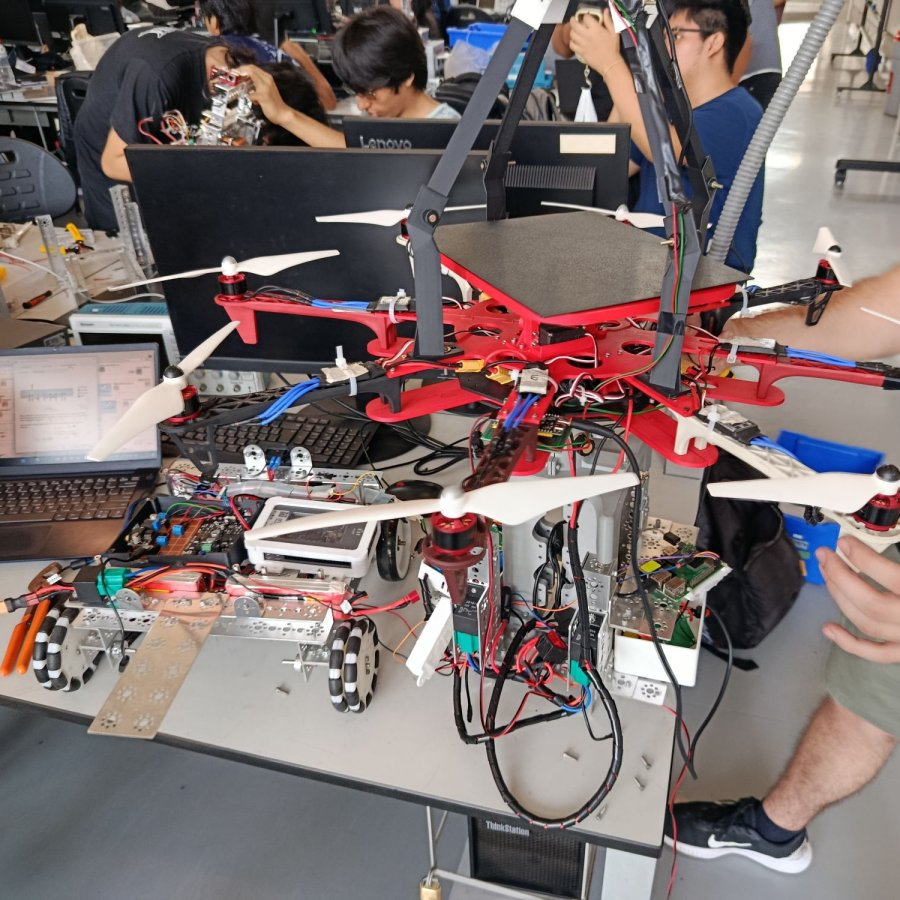
\includegraphics[width=\linewidth]{figures/paso7_integracion.jpg}\caption{Paso 8: integración.}\end{subfigure}
  \caption{Secuencia de construcción del prototipo final de AeroTray.}
  \label{fig:build}
\end{figure}

\begin{enumerate}[label=\textbf{Paso \arabic*.}, leftmargin=*, align=left]
  \item \textbf{Base móvil (Fig.~\ref{fig:build}a).}
  \begin{enumerate}[label=(\alph*)]
    \item Armar el chasis TETRIX con los dos motores TorqueNADO en el eje trasero y las ruedas omnidireccionales adelante.
    \item Medir la trocha (centro a centro de las ruedas motrices). Debe coincidir con el valor del nodo de fórmula de LabVIEW, \SI{0.3794}{\metre}.
    \item Cablear el motor izquierdo al MXP-A de la myRIO (PWM0 en el pin 27, dirección en DIO0, pin 11, encoder en ENC A/B) y el derecho al MXP-B con los mismos pines, a través del MDD10A.
    \item Proteger la NiMH con el fusible de \SI{20}{\ampere} y pasarla por el contacto del relé K3.
    \item \emph{Comprobación:} con las ruedas levantadas, ordenar avance y verificar que ambos contadores de encoder aumentan. El contador derecho se invierte por software.
  \end{enumerate}

  \item \textbf{Mástil, guía y rótula (Fig.~\ref{fig:build}b).}
  \begin{enumerate}[label=(\alph*)]
    \item Fijar el mástil vertical sobre el eje motriz y montar la guía vertical.
    \item Insertar el carro con la rótula esférica y verificar unos \SI{140}{\milli\metre} de recorrido libre.
    \item Poner topes blandos en ambos extremos de la guía.
    \item \emph{Comprobación:} el carro debe caer libremente por su propio peso; la fricción de la guía sesga la identificación por despegue de la Sección~\ref{sec:ident}.
  \end{enumerate}

  \item \textbf{Marco del octocóptero y alimentación (Fig.~\ref{fig:build}c).}
  \begin{enumerate}[label=(\alph*)]
    \item Imprimir la placa central y las torres (archivo\\ \fn{x8_UAV_R350_imprimible_bandeja_v5.stp}) y montar los ocho brazos cada \SI{45}{\degree}: M8 en $+x$, M7 en $+y$.
    \item Instalar M1--M4 con giro horario y M5--M8 con giro antihorario (Tabla~\ref{tab:params}).
    \item Armar las dos ramas de potencia independientes del esquema Rev.~I (Sección~\ref{sec:power}), cada una con LiPo, XT60, fusible ATO de \SI{30}{\ampere}, contacto 30--87 del relé (K1, K2), par trenzado 14\,AWG y condensador de \SI{1000}{\micro\farad} en el dron. La rama A alimenta los ESC 1, 3, 5 y 7, y la rama B los ESC 2, 4, 6 y 8; unir solo las tierras, y solo en el dron.
    \item Cortar el cable rojo (BEC) de los ESC.
    \item Conectar las señales de los ESC según la Tabla~\ref{tab:pins} (firmware v11): GPIO 25, 26, 27, 14, 21, 19, 5 y 17 para M1--M8 de la NodeMCU-32S; la MPU-6050 y el VL53L0X al I$^2$C (SDA 23, SCL 22).
    \item Alimentar la NodeMCU por el hub USB (dominio de lógica). No sumar un regulador desde la LiPo: serían dos fuentes de \SI{5}{\volt} en paralelo.
    \item Opcional, recomendado: soldar los divisores de VBAT hacia GPIO34/35 con R1 = R3 = \SI{10}{\kilo\ohm} y R2 = R4 = \SI{3.3}{\kilo\ohm} ($\div4{,}03$) y \SI{100}{\nano\farad} a GND, para que una versión futura del firmware mida la tensión (Sección~\ref{sec:bateria}).
  \end{enumerate}

  \item \textbf{Dron en la rótula (Fig.~\ref{fig:build}d).}
  \begin{enumerate}[label=(\alph*)]
    \item Atornillar el marco a la rótula de modo que el centro de la rótula coincida con el centro del marco.
    \item Equilibrar el conjunto: con los motores apagados debe quedar nivelado. Mover las baterías hasta lograrlo, y mantenerlas lo más bajas posible, porque la altura del centro de masa sobre la rótula fija la inestabilidad del módulo (Sección~\ref{sec:limits_fund}). El prototipo aún tiene una excentricidad residual de \SI{9.5}{\milli\metre} hacia M8, identificada en la Sección~\ref{sec:ident}.
  \end{enumerate}

  \item \textbf{Bandeja (Fig.~\ref{fig:build}e,f).}
  \begin{enumerate}[label=(\alph*)]
    \item Imprimir el plato, los mecanismos y las cuatro torres de la cámara.
    \item Montar los dos servos S3003 y conectar las señales a GPIO47 ($x$) y GPIO21 ($y$) de la ESP32-S3.
    \item Alimentar los servos desde el dominio S5 (BT6, XL4015, contacto de K4) con \SI{1000}{\micro\farad} en la entrada y tierra común con la ESP32-S3; no unir el pin de \SI{5}{\volt} de la ESP32-S3 a ese riel.
    \item Fijar la PS3 Eye en las torres, centrada sobre el plato, y ajustar el neutro del plato con los mecanismos hasta que quede nivelado en unos \SI{1390}{\micro\second}.
  \end{enumerate}

  \item \textbf{Supervisor y paro (Fig.~\ref{fig:build}g).}
  \begin{enumerate}[label=(\alph*)]
    \item Instalar Raspberry Pi OS (Debian 13) y crear un entorno virtual \texttt{\textasciitilde/venv} con \texttt{opencv-python}, \texttt{numpy}, \texttt{pyserial} y \texttt{esptool}.
    \item Copiar \texttt{pi\_control/} a la carpeta personal.
    \item Habilitar la UART física: en \texttt{raspi-config}, poner el \emph{login shell} serie en \emph{No} y el hardware serie en \emph{Sí}, y reiniciar.
    \item Cablear GPIO14 (TX, pin 8) al pin 10 (RX) del MXP-A, GPIO15 (RX, pin 10) al pin 14 (TX) del MXP-A, y tierra (pin 6) al pin 12 del MXP-A.
    \item Alimentar la Pi desde su propio pack 3S 18650 (BT5) y un XL4015 ajustado a \SI{5.2}{\volt}.
    \item Cablear la caja de mando: hongo SB1 (NC, enclavable) en serie con las bobinas de K1--K4 desde BT6 por un fusible de \SI{1}{\ampere}, con un diodo 1N4007 en antiparalelo con cada bobina. \emph{Comprobación:} con SB1 pulsado, ninguna rama debe tener tensión aguas abajo de su relé.
  \end{enumerate}

  \item \textbf{Firmware.}
  \begin{enumerate}[label=(\alph*)]
    \item Compilar el firmware del dron:\\ \texttt{arduino-cli compile --fqbn esp32:esp32:nodemcu-32s}.
    \item Grabarlo desde la Pi (\fn{cargar_vuelo_guia_desde_pi.sh}), que usa \texttt{esptool write-flash 0x0}.
    \item Grabar la ESP32-S3 con PlatformIO.
    \item Desplegar el proyecto de LabVIEW en la myRIO (\fn{prueba_prueba.vi} como VI principal).
  \end{enumerate}

  \item \textbf{Comprobaciones de integración (Fig.~\ref{fig:build}h).}
  \begin{enumerate}[label=(\alph*)]
    \item Lanzar \texttt{arrancar.sh} y abrir \url{http://<ip-de-la-pi>:8080/robot}. El registro debe mostrar el encabezado del firmware del dron, ``UART conectada en /dev/serial0'' y la tasa de la cámara.
    \item Con la batería desconectada, enviar \emph{cal} y verificar ``CAL OK''.
    \item Colocar la bola y verificar que se detecta en las cuatro esquinas del plato.
  \end{enumerate}
\end{enumerate}
